\ifdefined\activerhandout 
\documentclass[12pt,aspectratio=1610,handout]{beamer}
\else
\documentclass[12pt,aspectratio=1610]{beamer}
\fi

%\usepackage[french]{babel} %=> erreur avec les tikz du moteur
\usepackage[T1]{fontenc}
\usepackage[utf8]{inputenc}
\usepackage{lmodern}
\usepackage{hyperref}
\usepackage{smartdiagram}
\usepackage{tikz}
\usepackage{animate}
\usepackage{tikzpeople}
\usepackage{appendixnumberbeamer}
\usepackage[labelformat=empty]{caption}
%\usepackage{pictochrono}
\usepackage{fontawesome5}
\usepackage{awesomebox}

\usetheme{Warsaw}
\setbeamertemplate{page number in head/foot}[totalframenumber]

\newcommand{\anglais}[1]{(\textit{\color{blue}#1})}
\newcommand{\legende}[2]{\caption[#1 (Source : \cite{#2})]{#1}}
\newcommand{\histoire}[1]{\begin{awesomeblock}{2pt}{\faBook}{black!75}#1\end{awesomeblock}}
\newcommand{\info}[1]{\begin{awesomeblock}{2pt}{\faInfoCircle}{black!75}#1\end{awesomeblock}}
\newcommand{\question}[1]{\begin{awesomeblock}{2pt}{\faQuestionCircle}{black!75}#1\end{awesomeblock}}
\newcommand{\alerte}[1]{\begin{awesomeblock}{2pt}{\faExclamationCircle}{black!75}#1\end{awesomeblock}}
\newcommand{\astuce}[1]{\begin{awesomeblock}{2pt}{\faLightbulb}{black!75}#1\end{awesomeblock}}
\newcommand{\exemple}[1]{\begin{awesomeblock}{2pt}{\faSearch}{black!75}#1\end{awesomeblock}}
\newcommand{\definitionAConnaitre}[1]{\begin{awesomeblock}{2pt}{\faCog}{black!75}#1\end{awesomeblock}}

\newcommand{\qmcBia}[7]{
%1 : titre slide
%2 : numéro de la bonne réponse
%3 : Inititulé de la question
%4, 5, 6, et 7 : propositions de réponse
\begin{frame}{#1}
\begin{awesomeblock}{2pt}{\faQuestion}{black!75}
#3
	\begin{enumerate}
	\ifnum#2=1
		\only<1>{\item #4}
		\only<2>{\item \textbf{#4}}
	\else
		\item #4
	\fi
	\ifnum#2=2
		\only<1>{\item #5}
		\only<2>{\item \textbf{#5}}
	\else
		\item #5
	\fi
	\ifnum#2=3
		\only<1>{\item #6}
		\only<2>{\item \textbf{#6}}
	\else
		\item #6
	\fi
	\ifnum#2=4
		\only<1>{\item #7}
		\only<2>{\item \textbf{#7}}
	\else
		\item #7
	\fi
	\end{enumerate}
	\pause
\end{awesomeblock}
\end{frame}
}

\subtitle{BIA - Brevet d'Initiation Aéronautique}
\author{Clément \textsc{Vermot-Desroches}}
\institute{Collège Aliénor d'Aquitaine\\Martignas-sur-Jalle}
\date{\today}

%\AtBeginSection[]
%{
%    \begin{frame}
%        %\frametitle{Table of Contents}
%        \tableofcontents[currentsection]
%    \end{frame}
%}

\AtBeginSubsection[]
{
    \begin{frame}
        %\frametitle{Table of Contents}
        \tableofcontents[currentsection,currentsubsection]
    \end{frame}
}

\title[Séance 4 - Commandes de vol]{Séance 4 \\ Commandes de vol}

\begin{document}
 \begin{frame}
 \titlepage
 \end{frame}
 
 \begin{frame}
 \tableofcontents
 \end{frame}
 
 \section{Les axes}
	\begin{frame}{Axes - Question}
	
	\question{Sur quels axes peut évoluer un aéronef ?}
	\pause
	\question{Comment le pilote peut-il intervenir sur ces axes ?}
	\pause
	\question{Qu'es-ce qui permet, sur l'aéronef, d'agir sur ces axes ?}
	\end{frame}	 

 	\begin{frame}{Les axes sur un aéronef}
		\begin{figure}[H]
  			\only<1>{\includegraphics[scale=1]{imgPresentations/axes.pdf}}
  			\only<2>{\includegraphics[scale=1]{01-EtudeAeronefs/img/axes.pdf}}
  			\legende{Les axes sur un aéronef}{img:axes}	
  			\pause
		\end{figure}
	\end{frame}	
	
\section{Commandes de vol}
	\begin{frame}{Commandes de vol - axes du roulis}
	\begin{columns}
 	\begin{column}{0.5\textwidth}
	La commande sur l'axe du roulis (inclinaison gauche-droite) est obtenue par :
	\begin{itemize}
		\item une action latérale sur le manche
		\item provoquant un déplacement des ailerons
		\item montée de l'aileron du côté du virage, descente de l'aileron opposé.
	\end{itemize}
	\end{column}
	\begin{column}{0.5\textwidth}
		\begin{figure}[H]
  			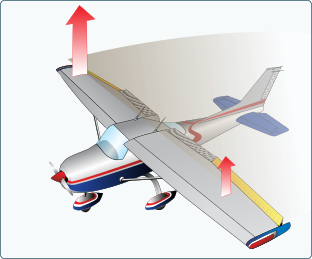
\includegraphics[width=1\textwidth]{01-EtudeAeronefs/img/virage.pdf}
  			\legende{Mise en virage à gauche}{img:virage}	
		\end{figure}	
	\end{column}
	\end{columns}
	\end{frame}
	
	\begin{frame}{Commandes de vol - axes du roulis - lacet inverse}
	\begin{columns}
	\begin{column}{0.5\textwidth}
		\begin{figure}[H]
  			\includegraphics[width=1\textwidth]{01-EtudeAeronefs/img/lacetInverse.pdf}
  			\legende{Lacet inverse (à droite pour un virage à gauche)}{img:lacetInverse}	
		\end{figure}	
	\end{column}
 	\begin{column}{0.5\textwidth}
	La trainée supplémentaire créée par l'augmentation de la portance provoque un lacet dans sens inverse au virage
	\end{column}
	\end{columns}
	\end{frame}
	
	\begin{frame}{Commandes de vol - axes du tangage}
	\begin{columns}
 	\begin{column}{0.5\textwidth}
	La commande sur l'axe du tangage (avant arrière) est obtenue par :
	\begin{itemize}
		\item une action longitudinale sur le manche
		\item provoquant un déplacement de la gouverne de profondeur
		\item la gouverne monte quand on tire sur la manche, et descend quand on pousse.
	\end{itemize}
	\end{column}
	\begin{column}{0.5\textwidth}
		\begin{figure}[H]
  			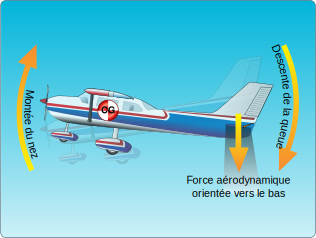
\includegraphics[width=1\textwidth]{01-EtudeAeronefs/img/gouverneProfondeur.pdf}
  			\legende{Commande de profondeur}{img:gouverneProfondeur}	
		\end{figure}	
	\end{column}
	\end{columns}
	\end{frame}
	
	\begin{frame}{Commandes de vol - axes du lacet}
	\begin{columns}
	\begin{column}{0.5\textwidth}
		\begin{figure}[H]
  			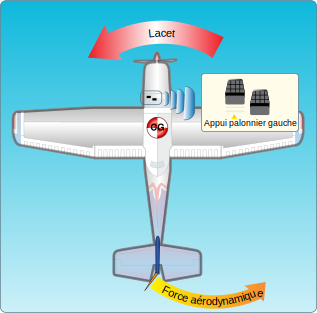
\includegraphics[width=1\textwidth]{01-EtudeAeronefs/img/gouverneDeDirection.pdf}
  			\legende{Commande de profondeur}{img:gouverneDeDirection}	
		\end{figure}	
	\end{column}
	\begin{column}{0.5\textwidth}
	La commande sur l'axe du lacet (latéral) est obtenue par :
	\begin{itemize}
		\item une action sur le palonnier (pédale)
		\item provoquant un déplacement de la gouverne de direction
		\item la gouverne se déplace du côté de l'appui.
	\end{itemize}
	\end{column}
	\end{columns}
	\end{frame}
 
 
\appendix 
\section{QCM}
%\qmcBia{Étude des aéronefs}
%{3}{\begin{figure}[H]
%  		\centering
%    		\includegraphics[width=0.2\textwidth]{01-EtudeAeronefs/img/PWWasp.jpg}
%	\end{figure}	
%	La disposition des cylindres de ce moteur est :}
%{en ligne}
%{en V}
%{en étoile}
%{à plat} 



 
\ifdefined\activerbibliobeamer
\begin{frame}[allowframebreaks]
\frametitle{Bibliographie}
\printbibliography
%\nocite{*}
\end{frame}
\fi 
 
\end{document}
